\documentclass{beamer}


\usepackage{amssymb,amsmath}
\usepackage{graphicx}
\usepackage{url}
\usepackage{color}
\usepackage{relsize}		% For \smaller
\usepackage{url}			% For \url
\usepackage{epstopdf}	% Included EPS files automatically converted to PDF to include with pdflatex

%For MindMaps
% \usepackage{tikz}%
% \usetikzlibrary{mindmap,trees,arrows}%

%%% Color Definitions %%%%%%%%%%%%%%%%%%%%%%%%%%%%%%%%%%%%%%%%%%%%%%%%%%%%%%%%%
%\definecolor{bordercol}{RGB}{40,40,40}
%\definecolor{headercol1}{RGB}{186,215,230}
%\definecolor{headercol2}{RGB}{80,80,80}
%\definecolor{headerfontcol}{RGB}{0,0,0}
%\definecolor{boxcolor}{RGB}{186,215,230}

%%% Save space in lists. Use this after the opening of the list %%%%%%%%%%%%%%%%
%\newcommand{\compresslist}{
%	\setlength{\itemsep}{1pt}
%	\setlength{\parskip}{0pt}
%	\setlength{\parsep}{0pt}
%}

%\setbeameroption{show notes on top}

% You should run 'pdflatex' TWICE, because of TOC issues.

% Rename this file.  A common temptation for first-time slide makers
% is to name it something like ``my_talk.tex'' or
% ``john_doe_talk.tex'' or even ``discrete_math_seminar_talk.tex''.
% You really won't like any of these titles the second time you give a
% talk.  Try naming your tex file something more descriptive, like
% ``riemann_hypothesis_short_proof_talk.tex''.  Even better (in case
% you recycle 99% of a talk, but still want to change a little, and
% retain copies of each), how about
% ``riemann_hypothesis_short_proof_MIT-Colloquium.2000-01-01.tex''?

\mode<presentation>
{
  % A tip: pick a theme you like first, and THEN modify the color theme, and then add math content.
  % Warsaw is the theme selected by default in Beamer's installation sample files.

  %%%%%%%%%%%%%%%%%%%%%%%%%%%% THEME
  %\usetheme{AnnArbor}
  %\usetheme{Antibes}
  %\usetheme{Bergen}
  %\usetheme{Berkeley}		% bem bacana - menu esquerdo
  %\usetheme{Berlin}
  %\usetheme{Boadilla}
  %\usetheme{boxes}
  %\usetheme{CambridgeUS}		% bem bacana - menu superior
  %\usetheme{Copenhagen}
  %\usetheme{Darmstadt}
  %\usetheme{default}
  %\usetheme{Dresden}
  \usetheme{Frankfurt}
  %\usetheme{Goettingen}
  %\usetheme{Hannover}		% bem bacana - menu esquerdo
  %\usetheme{Ilmenau}
  %\usetheme{JuanLesPins}
  %\usetheme{Luebeck}
  %\usetheme{Madrid}		%bacana
  %\usetheme{Malmoe}
  %\usetheme{Marburg}		% bem bacana - menu direito
  %\usetheme{Montpellier}
  %\usetheme{PaloAlto}		% bem bacana - menu esquerdo
  %\usetheme{Pittsburgh}
  %\usetheme{Rochester}		%bacana
  %\usetheme{Singapore}
  %\usetheme{Szeged}
  %\usetheme{Warsaw}

  %%%%%%%%%%%%%%%%%%%%%%%%%%%% COLOR THEME
  %\usecolortheme{albatross}		% azul escuro, massa
  %\usecolortheme{beetle}		% cinza, menu azul
  %\usecolortheme{crane}		% branco e amarelo, massa
  \usecolortheme{default}		% branco, azul clarinho
  %\usecolortheme{dolphin}		% azul e branco, legal
  %\usecolortheme{dove}			% cinza e branco, feio
  %\usecolortheme{fly}			% todo cinza, horrível
  %\usecolortheme{lily}			% parece o default
  %\usecolortheme{orchid}		% azul e branco, ok
  %\usecolortheme{rose}			% branco e violeta-claro, bonito
  %\usecolortheme{seagull}		% cinza, feio
  %\usecolortheme{seahorse}		% nhé, meio feio
  %\usecolortheme{sidebartab}		% Azul, branco, destaque na tab, interessante
  %\usecolortheme{structure}		% bichado
  %\usecolortheme{whale}		% Azul e branco, bem bonito

  %%%%%%%%%%%%%%%%%%%%%%%%%%%% OUTER THEME
  \useoutertheme{default}
  %\useoutertheme{infolines}
  %\useoutertheme{miniframes}
  %\useoutertheme{shadow}
  %\useoutertheme{sidebar}
  %\useoutertheme{smoothbars}
  %\useoutertheme{smoothtree}
  %\useoutertheme{split}
  %\useoutertheme{tree}

  %%%%%%%%%%%%%%%%%%%%%%%%%%%% INNER THEME
  \useinnertheme{circles}
  %\useinnertheme{default}
  %\useinnertheme{inmargin}
  %\useinnertheme{rectangles}
  %\useinnertheme{rounded}

  %%%%%%%%%%%%%%%%%%%%%%%%%%%%%%%%%%%

  \setbeamercovered{invisible} % or whatever (possibly just delete it)
  % To change behavior of \uncover from graying out to totally
  % invisible, can change \setbeamercovered to invisible instead of
  % transparent. apparently there are also 'dynamic' modes that make
  % the amount of graying depend on how long it'll take until the
  % thing is uncovered.

}


% Get rid of nav bar
\beamertemplatenavigationsymbolsempty

% Use short top
%\usepackage[headheight=12pt,footheight=12pt]{beamerthemeboxes}
%\addheadboxtemplate{\color{black}}{
%\hskip0.5cm
%\color{white}
%\insertshortauthor \ \ \ \ 
%\insertframenumber \ \ \ \ \ \ \ 
%\insertsection \ \ \ \ \ \ \ \ \ \ \ \ \ \ \ \ \  \insertsubsection
%\hskip0.5cm}
%\addheadboxtemplate{\color{black}}{
%\color{white}
%\ \ \ \ 
%\insertsection
%}
%\addheadboxtemplate{\color{black}}{
%\color{white}
%\ \ \ \ 
%\insertsubsection
%}

% Insert frame number at bottom of the page.
% \usefoottemplate{\hfil\tiny{\color{black!90}\insertframenumber}} 

\usepackage[english]{babel}
\usepackage[latin1]{inputenc}
\usepackage{subfigure}

\usepackage{times}
\usepackage[T1]{fontenc}


\title[GB21802]{GB21802 - Programming Challenges}
\subtitle[]{Week 0 - Introduction}
\author[Claus Aranha]{Claus Aranha\\{\footnotesize caranha\@@cs.tsukuba.ac.jp}}
\institute{Department of Computer Science}
\date{2018/4/13\\{\smaller(last updated: \today)}}

\begin{document}

\section{Introduction}
\subsection{About the Course}

\begin{frame}
\maketitle
\end{frame}


\begin{frame}
  \frametitle{Before Anything else: Important Notices}

  \begin{block}{Manaba Page}
    All lecture notes and announcements for this course will be done
    through MANABA. Access the url below:
    
    \medskip
    
    \url{https://manaba.tsukuba.ac.jp/ct/course_971789}\\
    Registration Code: 1473177
  \end{block}
  \begin{exampleblock}{Language}
    \begin{itemize}
      \item Lectures: Japanese
      \item Slides and materials: English
      \item Exercises: English
      \item Questions, Mails and Homework: Any language
    \end{itemize}
  \end{exampleblock}
\end{frame}

\begin{frame}
  \frametitle{About the Lecturer}
  \begin{columns}
    \column{0.4\textwidth}
    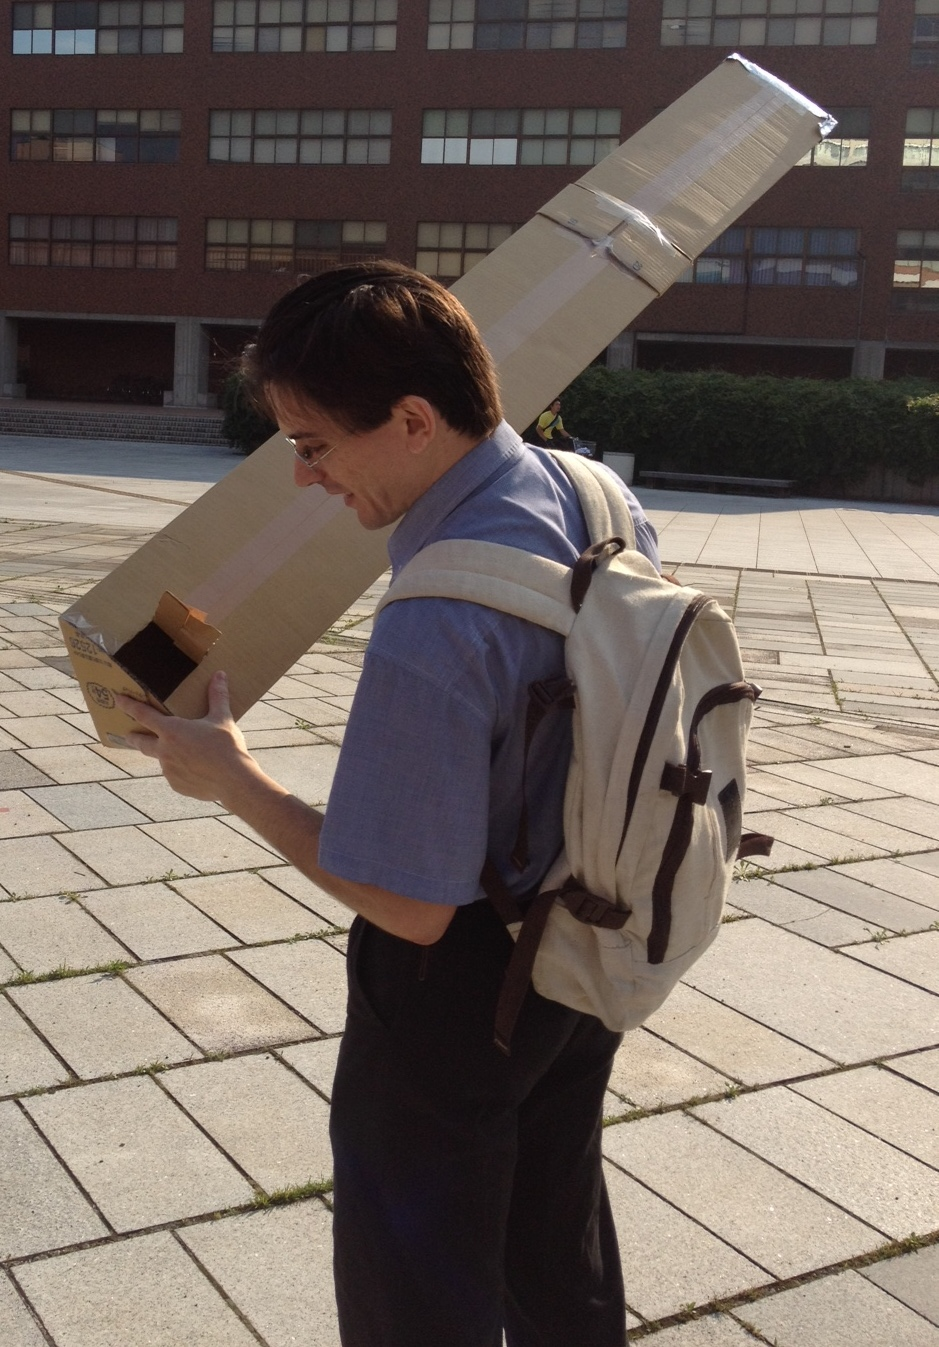
\includegraphics[width=1\textwidth]{../img/pinhole}
    \column{0.6\textwidth}
    {\small
    \begin{itemize}
      \item \structure{Name:} Claus Aranha;
      \item \structure{Country:} Brazil;
        
        \medskip

      \item \structure{Research:} Artificial Intelligence,
        Evolutionary Algorithms, Genetic Programming;
      \item \structure{Language:} Python, R;
      \item \structure{Hobbies:} Game Programming, Geocaching;
        
        \medskip

      \item \structure{webpage:}\\ {\smaller \url{http://conclave.cs.tsukuba.ac.jp}}
    \end{itemize}
    }
  \end{columns}
\end{frame}

\begin{frame}
  \frametitle{What is this course about?}
  
  You have learned many programming techniques...\\\hfill ...but can you use them?

  \begin{block}{Course Philosophy: Learning by Practice}
    \begin{itemize}
      {\small
    \item Every week, you will be asked to solve some programming
      problems;
    \item You have to decide the best \structure{data structure}, and
      \structure{algorithm} to solve each problem;
    \item Each problem has a \alert{max time}, and \alert{max memory};
    \item We will discuss algorithms, techniques and tricks;
      }
    \end{itemize}
  \end{block}

  \begin{exampleblock}{Course Goal:}
    Improve programming abilities, techniques and familiarity.
  \end{exampleblock}
\end{frame}

\begin{frame}
  \frametitle{Why you should do this class?}
  \begin{itemize}
  \item \structure{You like to program, you think programming is fun}

    \smallskip
    
  \item You learned a lot of programming theory, but you need more
    programming practice;
    
    \smallskip

  \item You have not written many programs yet;

    \smallskip

  \item You want to think about program efficiency;

    \smallskip

  \item You want a class where skill is more important than memorization;

    \smallskip

  \item You want to practice your technical English;

    \smallskip

  \item You want to participate in Programming Contests;
  \end{itemize}
\end{frame}

\begin{frame}
  \frametitle{Warnings about this class}
  \begin{alertblock}{1- Heavy Workload}
    \begin{itemize}
    \item Challenges start easy, but end very hard;
    \item Expect to use a few hours per week on homework;
    \item Lots of debugging;

      \bigskip

    \item Hint: Do your homework early!
    \end{itemize}
  \end{alertblock}

  \begin{alertblock}{2- Course Language}
    \begin{itemize}
    \item The teacher's Japanese is very bad T\_T
    \item All the course materials are in English;
    \item Importantly: All the homework is in English;
    \item You can make your homework in Japanese;

      \bigskip

    \item Practice some English in this course too! :-)
    \end{itemize}
  \end{alertblock}

\end{frame}

\section{Programming Challenges}
\subsection{Example}

\begin{frame}
  \frametitle{What is a ``Programming Challenge''?}

  A programming challenge is a puzzle that you solve by making a
  computer program.

  \bigskip

  \begin{itemize}
  \item Description of the problem
  \item Standard input
  \item Standard output
  \item Examples
  \end{itemize}
  
  \bigskip

  You must write a program that \structure{reads the input} and
  \structure{prints the correct output}.
  
\end{frame}

\begin{frame}
  \frametitle{Example Challenge: ``Relational Operator'' (1)}

  {\small
  The challenges for this course are listed at the page:\\
  {\smaller \url{http://conclave.cs.tsukuba.ac.jp/lecture/monitor.html}}

  \begin{center}
    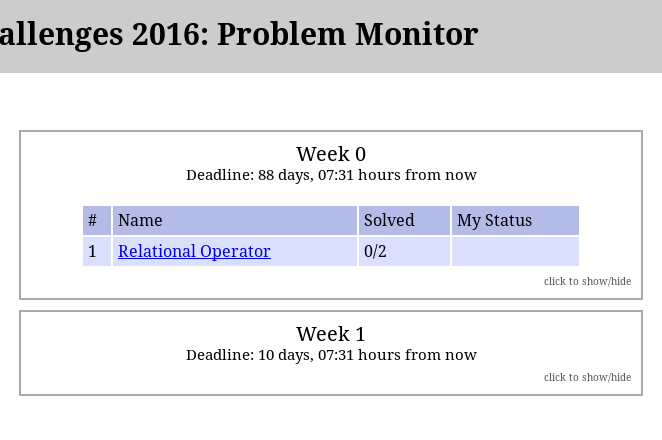
\includegraphics[width=.7\textwidth]{../img/monitorpage}
  \end{center}

  Click on the title to go to the problem page.}
\end{frame}

\begin{frame}
  \frametitle{Example Challenge: ``Relational Operator'' (2)}

  Clicking on the title will take you to the problem page.
  
  \begin{center}
    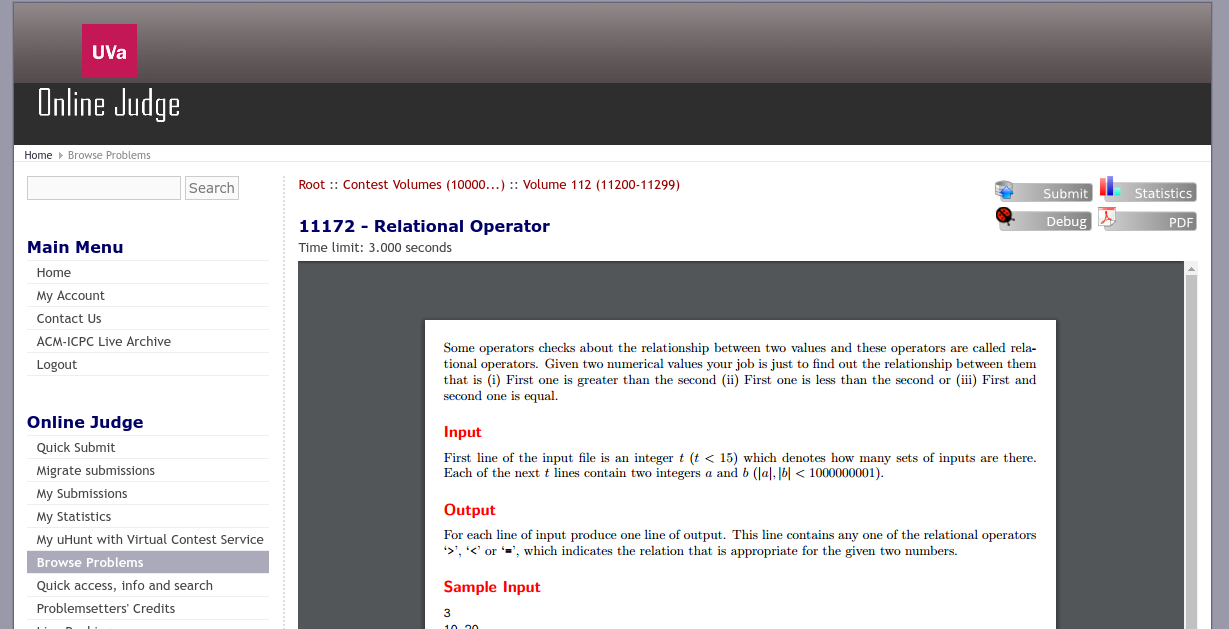
\includegraphics[width=.9\textwidth]{../img/relationaloperator}
  \end{center}

  Here you can read the problem and submit a solution.\\
  (You will need an UVA account!)

\end{frame}

\begin{frame}
  \frametitle{Example Challenge: ``Relational Operator'' (3)}
  
  \begin{block}{Problem Description}
    {\smaller Some operator checks about the relationship between two
      values, these operators are called relational operators. Given
      \structure{two numerical values}, your job is just to find out
      the relationship between them.
      \begin{itemize}
      \item First one is greater than the second
      \item First one is smaller than the second
      \item First one is equal to the second
      \end{itemize}
    }
  \end{block}
  \begin{block}{Input}
    {\smaller
      First line is the number $t$ of tests ($t < 15$). Following t lines 
      are two integers $a$ and $b$.
    }
  \end{block}
  \begin{block}{Output}
    {\smaller
      For each line of input, print one line of output with '>','<' or '=', 
      according to the relationship of $a$ and $b$.
    }
  \end{block}
\end{frame}



\begin{frame}[fragile]
  \frametitle{Solving ``Relational Operator''}
    
\begin{block}{}
{\smaller
\begin{verbatim}
// UVA 11172 - Relational Operator
// Test if a is bigger, smaller or equal to b

#include <iostream>
using namespace std;

int main()
{
    int n; long a, b;

    cin >> n;    
    for (; n > 0; n--)
    {
        cin >> a >> b;
        if (a > b) cout << ">\n";
        if (a < b) cout << "<\n";
        if (a == b) cout << "=\n";
    }
}
\end{verbatim}}
\end{block}
\end{frame}

\begin{frame}[fragile]
  \frametitle{A Python Solution (python 3)}
  \begin{block}{}
\begin{verbatim}
n = int(input())

while (n > 0):
   line = input()
   tokens = line.split()
   a,b = int(tokens[0]),int(tokens[1])

   if a > b: print(">")
   if a < b: print("<")
   if a == b: print("=")

   n -= 1
\end{verbatim}
  \end{block}
  
\end{frame}

\begin{frame}[fragile]
  \frametitle{A Java Solution}

  {\tiny
  \begin{block}{}
\begin{verbatim}
import java.io.*;
class Main
{
   public static void main(String args[])
   {
      BufferedReader stdin = new BufferedReader(new InputStreamReader(System.in));
      BufferedWriter stdout = new BufferedWriter(new OutputStreamWriter(System.out));
      try {
      String line;
      line = stdin.readLine();      
      int n = Integer.parseInt(line);
      
      for (int i = 0; i < n; i++)
      {
         line = stdin.readLine();
         String[] tokens = line.split("\\s+");
         long a = Integer.parseInt(tokens[0]);
         long b = Integer.parseInt(tokens[1]);
         
         if (a > b)
            stdout.write(">\n");
         if (a < b)
            stdout.write("<\n");
         if (a == b)
            stdout.write("=\n");
         stdout.flush();
      }
      stdout.close();
      } catch (IOException ioe) { System.out.println("I/O Exception");}
   }
}
\end{verbatim}
  \end{block}
  }
\end{frame}

\begin{frame}
  \frametitle{Java Solution -- Keep in Mind}

  \begin{itemize}
  \item All code must be in the same source file (can define many
    classes in this file)

    \medskip

  \item All programs must begin in a static main method in a
    \structure{Main} class.

    \medskip

  \item Do not use public classes. Even Main must be non public.

    \medskip

  \item Use Buffered I/O to avoid time limit exceeded.
  \end{itemize}
\end{frame}




\subsection{Submission}

\begin{frame}
  \frametitle{How to submit a problem} 
  
  Your weekly routine should have five steps:

  \begin{enumerate}
  \item Read the problem and think how to solve it;
    \medskip
    
  \item Write the program, and submit it to UVA website;
    \medskip
    
  \item If the program is correct go to 4, else go to 2;
    \medskip
    
  \item Prepare your source zip file (all code + comment file);
    \medskip
    
  \item Submit your zip file to MANABA;
  \end{enumerate}
\end{frame}

\begin{frame}
  \frametitle{Submitting the problem to UVA}

  {\small
  UVA is an \structure{Automated Robotic Judge}. It will test your
  program on a set of inputs, and check if the outputs are correct.

  \medskip
  
  From the problem page, click on the \structure{submit} button. 
  
  \begin{center}
    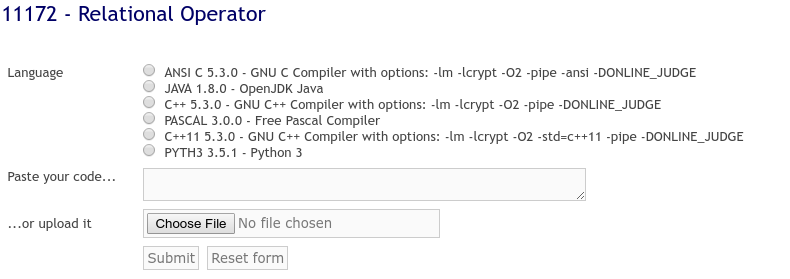
\includegraphics[width=.8\textwidth]{../img/submitpage}
  \end{center}
  
  Select your language, choose the file, and press submit.\\
  (You can use C, C++, Java, Python {\tiny and Pascal})}
\end{frame}

\begin{frame}
  \frametitle{Submitting the problem to UVA}

  {\small

    After you submit the program, the judge gives you the result
    (Verdict) and the Run time.
    
    \begin{center}
      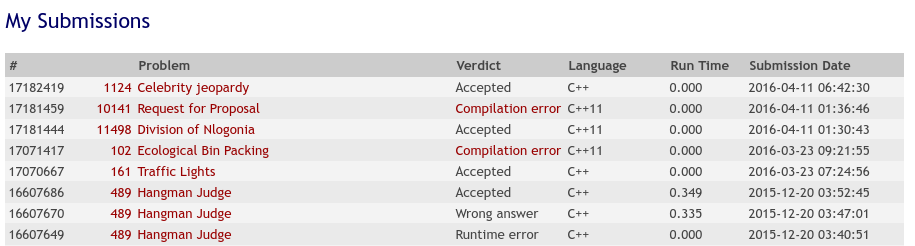
\includegraphics[width=.8\textwidth]{../img/submissionpage}
    \end{center}

    You can see this information on the ``my submissions'' page.
  }
\end{frame}

\begin{frame}
  \frametitle{Submission Statues:}
  \begin{itemize}
  \item \structure{Accepted}: Your program is correct!
    Congratulations!

    \bigskip
    
  \item \structure{Wrong Answer}: Your program is incorrect. Debugging
    time.

    \bigskip

  \item \structure{Time/Memory limit exceeded}: Your program is
    inefficient. You need a better algorithm.

    \bigskip
  \item \structure{Runtime Error}: Your program is crashing. To the
    debugger!

    \bigskip
  \end{itemize}

\end{frame}

\begin{frame}
  \frametitle{Back to the problem Monitor}

  In the problem monitor page, you can check how many people solved
  each problem, which problems you still have to solve, and the
  deadlines.

  \begin{center}
    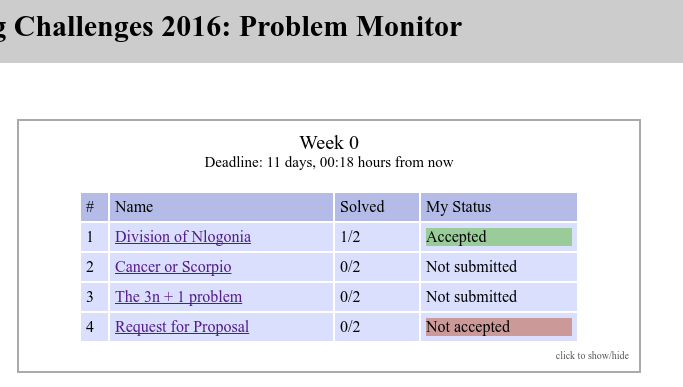
\includegraphics[width=.7\textwidth]{../img/monitorpage2}
  \end{center}
\end{frame}

\subsection{Manaba Submission}
\begin{frame}
  \frametitle{Submitting the problem to MANABA}

  {\small
  After you finish the problems listed in the monitor, you need to
  submit your source code and a comment file as a zip package to MANABA.}

  \medskip

  {\small
  \begin{columns}
    \column{0.3\textwidth}
    \column{0.4\textwidth}
    \begin{block}{s2015XXXXXX-weekYY.zip}
      \begin{itemize}
      \item problem1.cpp
      \item problem2.cpp
      \item problem5.cpp
      \item kaisetsu.txt
      \end{itemize}
    \end{block}
    \column{0.3\textwidth}
  \end{columns}
  }

  \medskip
  
  \begin{alertblock}{Attention}
  Submission to the UVA judge without a submission to MANABA will not
  be accepted!
  \end{alertblock}
\end{frame}

\section{Course Rules}
\subsection{Course Structure}

\begin{frame}
    \frametitle{Outline}
    
    \begin{block}{Two classes per week}
        \begin{itemize}   
        \item Each week has a theme
        \item Friday Class: Introduction
        \item Monday Class: Problem Solving and Q\&A
        \end{itemize}
    \end{block}
    
    \begin{block}{Solving Problems}
        \begin{itemize}
        \item Every week there are 6-10 programming assignments;
        \item Assignments follow the weekly theme;
        \item Automatic Submission and Evaluation System;
        \item Program Deadline is Thursday 23:59
        \end{itemize}
    \end{block}
\end{frame}
    
\begin{frame}
  \frametitle{Outline}
  \begin{center}
    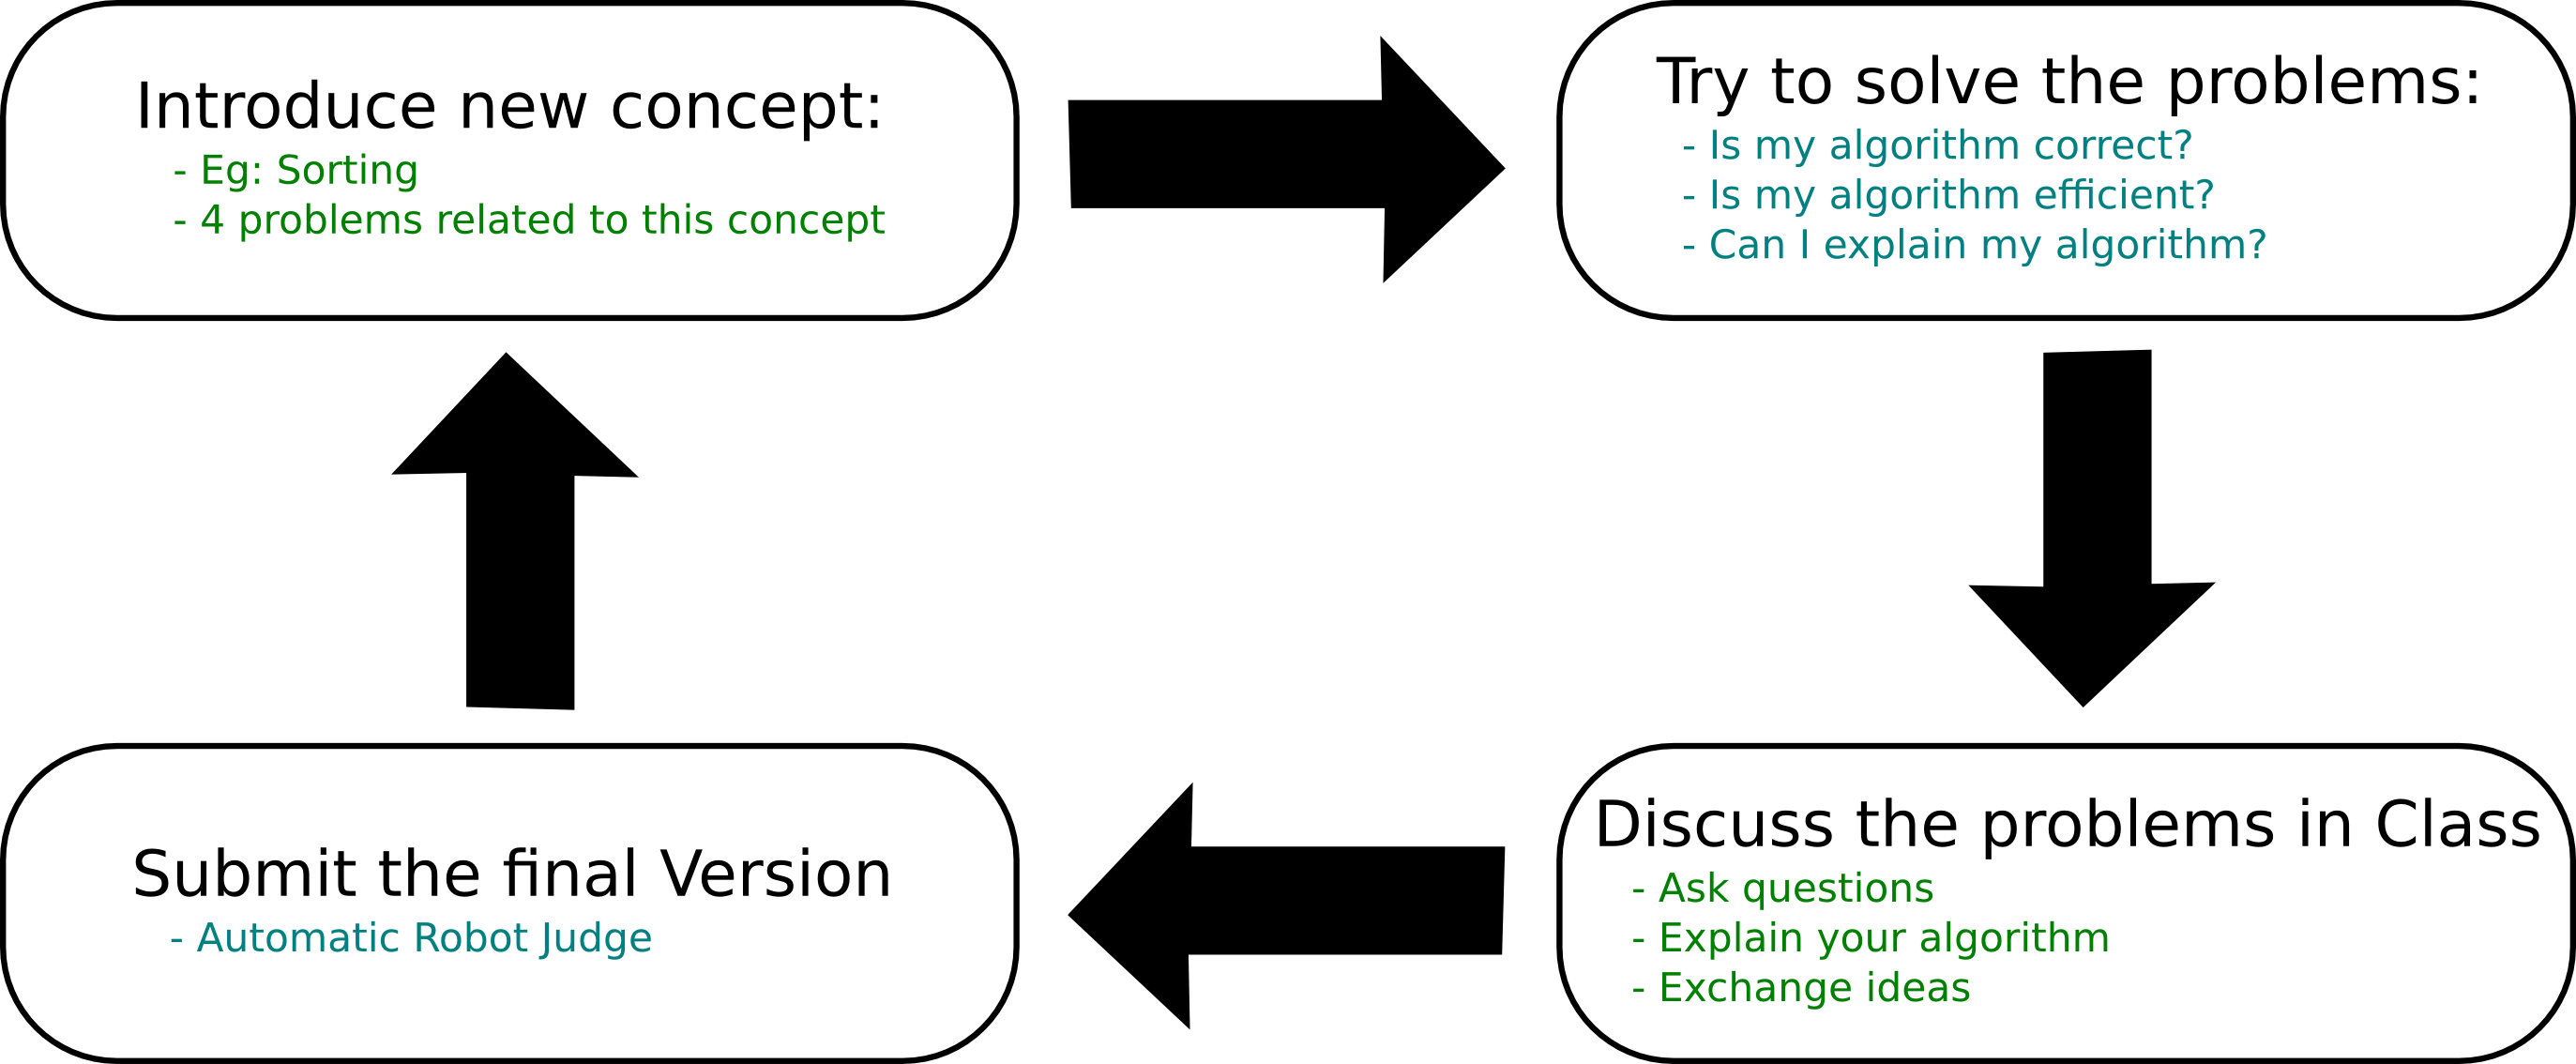
\includegraphics[width=1\textwidth]{../img/classoutline}
  \end{center}
\end{frame}

\subsection{Grading}

\begin{frame}
  \frametitle{Evaluation and Grading (1)}

  Evaluation Criteria: \structure{Problems solved}, \structure{Code}
  and \structure{Participation}
  
  \bigskip

  Evaluation Process: Base Grade \structure{+Bonus} \alert{-Penalty}
\end{frame}

\begin{frame}
  \frametitle{Evaluation and Grading (2) -- Base Grade}

  The \structure{Base Grade} is based on homework submissions to UVA.

  \bigskip
  
  \begin{itemize}
  \item \structure{C}: You Solved One problem every week;

    \medskip

  \item \structure{B}: You Solved Two problems every week;

    \medskip

  \item \structure{A}: You Solved Three problems every week;
  \end{itemize}

\end{frame}

\begin{frame}
  \frametitle{Evaluation and Grading (3) -- Bonus and Penalty}
  
  {\small
  A \structure{Bonus} or \structure{Penalty} will be added to the base grade.
  \begin{itemize}
    \item Bonus: grade one step up (C->B, B->A, A->A+)
    \item Penalty: grade one step down (A+->A, B->C, \alert{C->C})
  \end{itemize}
  }

  \medskip
  \begin{exampleblock}{Bonus: Grade Up}
    \begin{itemize}
    \item Students with the largest number of solutions in each
        category (A,B,C)
    \item Students with exceptional comment files
    \item Great participation in Class
    \end{itemize}
  \end{exampleblock}
  \begin{alertblock}{Penalty: Grade Down}
    \begin{itemize}
    \item More than 25\% problems submitted after the deadline
    \end{itemize}
  \end{alertblock}

  \tiny{Parameter $N$ will be decided at a later date.}
\end{frame}

\begin{frame}[fragile]
  \frametitle{Evaluation and Grading (4) -- comment/kaisetsu file}

  When you submit your package every week, include a text file (no
  Word!) with comments on each problem you tried to solve.
    
  \begin{exampleblock}{Example}
    {\smaller
\begin{verbatim}
Name: Claus, ID: 98884735
# Problem 1:
To solve this problem, I sorted the input data, and 
printed the input with the highest number of repeated 
letters.

# Problem 2: 
I tried to solve this problem with brute force, but 
the time limit was exceeded. I had to use DP on the 
number of people instead.
\end{verbatim}}
  \end{exampleblock}

  \bigskip
  
  Comments may be in Japanese. {\small (FILENAMES must be in romaji)}
\end{frame}

\begin{frame}
  \frametitle{Evaluation and Grading (5) -- about plagiarism}
  
  The assignments are \alert{individual}. Use your \structure{own
    strength} to solve the programs.

  \begin{exampleblock}{GOOD}
    \begin{itemize}
    \item Ask for ideas to your friends;
    \item Ask for ideas in the MANABA forum;
    \item Ask for help with a bug;
    \end{itemize}
  \end{exampleblock}

  \begin{alertblock}{BAD}
    \begin{itemize}
    \item Copy a solution from the internet;
    \item Copy a solution from your friends;
    \item Give your code to a friend;
    \end{itemize}
  \end{alertblock}

  Plagiarism will result in course failure, and possibly worse.
\end{frame}

\section{Resources}
\subsection{Resources}

% Class Links
\begin{frame}
  \frametitle{Useful Links}
  \begin{itemize} 
  \item
    \href{https://manaba.tsukuba.ac.jp/ct/course_971789}
         {\structure{\underline{Manaba Page}}}: All the class material
         will be here. Access Code is: 1473177

    \medskip

  \item \href{https://uva.onlinejudge.org/}{\structure{\underline{UVA Online Judge}}}:
    Use this page to submit your problems. \alert{Make an account and list the username on MANABA}

    \medskip

  \item \href{https://conclave.cs.tsukuba.ac.jp/lecture/monitor.html}{\structure{\underline{Problem Monitor}}}:
    Use this page to check deadlines and weekly problems.

    \medskip

  \item
    \href{https://www.github.com/caranha/ProgrammingChallengesLectureNotes}{\structure{\underline{Github
          Repository}}}:
    Working directory for lecture notes. Send me PR, issues!

    \medskip
    
  \item
    \href{https://www.udebug.com/}{\structure{\underline{uDebug}}}:
    Web service that generates test inputs and test outputs for UVA
    problems. Useful tool for this course.
  \end{itemize}
\end{frame}


% Books
% TODO: Add japanese books % Needs CJK package (or book images)
\begin{frame}
  \frametitle{Course Book}

  \begin{itemize}
  \item Competitive Programming, 3rd Edition
    (\href{http://cpbook.net/}{http://cpbook.net})
    
    \bigskip

  \item For suggestions of books in Japanese, please check the Manaba materials!
  \end{itemize}
\end{frame}

% udebug
\begin{frame}
  \frametitle{uDebug Tool}

  If you are having problems, the uDebug site offers, for many
  problems in UVA, the correct set of outputs for any input you give.

  \bigskip

  \url{https://www.udebug.com/}

  \bigskip

  \begin{center}
    
\includegraphics[width=0.7\textwidth]{../img/udebug}
  \end{center}
\end{frame}

% Cat stream
\begin{frame}
  \frametitle{If you are still having problems...}

  Watch a cat stream to relax!

  \bigskip

  \begin{center}
    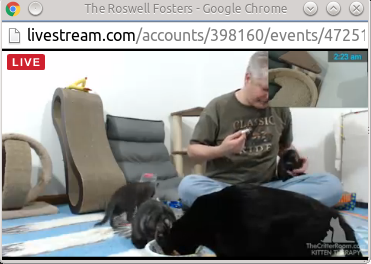
\includegraphics[width=.6\textwidth]{../img/catstream}
  \end{center}

  \bigskip

  \url{http://livestream.com/FosterKittenCam/}
\end{frame}


% Contact the professor (e-mail, twitter, webpage, room)
\begin{frame}
  \frametitle{Contact the professor}
  \begin{itemize}
  \item \structure{e-mail}: caranha@cs.tsukuba.ac.jp
  \item \structure{website}: \url{http://conclave.cs.tsukuba.ac.jp}
  %\item \structure{twitter}: @caranha

    \bigskip

  \item \structure{Room}: SB1012 -- Send an e-mail and we can talk!\\
  \end{itemize}

  \bigskip

  Both English and Japanese are okay!
\end{frame}


% Do we still have time? Fill out the forms!
% Do we still have time? Ask me questions!

\begin{frame}
  \frametitle{Do we still have some time?}

  \begin{itemize}
  \item Create an account on UVA (if you already have an account, you can use that)

    \bigskip

  \item Submit your account name to the MANABA

    \bigskip

  \item Ask any other questions you want to know!
  \end{itemize}

  \bigskip

  \begin{center}
    Thank you for today!
  \end{center}
\end{frame}

\end{document}
